\documentclass{article}
\title{Matrix Equation Solvers}
\author{Alex Harvey - mm13ah - ID: 200786528}
\date{}

\usepackage{amsmath}
\numberwithin{equation}{section}
\usepackage{amssymb}
\usepackage{amsthm}
\usepackage{blindtext}
\usepackage[parfill]{parskip}
\usepackage{graphicx}
\usepackage{textcomp}
\usepackage[utf8]{inputenc}
\usepackage{float}
\usepackage{diagbox}
\usepackage{tikz}
\usepackage{pgfgantt}
\usepackage{nicefrac}
\usepackage{caption}

\newcommand{\subsubsubsection}[1]{\paragraph{#1}\mbox{}\\}
\setcounter{secnumdepth}{4}
\setcounter{tocdepth}{4}

\begin{document}

\maketitle

\newpage

\tableofcontents

\clearpage

\section{Introduction}
\subsection{Problem Statement}

The traditional approach to solving partial differential equations (PDEs) numerically involves stacking all the unknowns of the problem into a single vector which ignores underlying structures. This prevents methods from being used which can take advantage of the problem structure to solve the problem more efficiently. This can come at a significant cost when uncertainty is introduced into the problem. An alternative approach is to formulate the problem as a matrix equation, which can be solved using a range of different methods. This project involves exploring methods that solve this alternative formulation and how these solvers compare against each other. 

As an example, define spatial domain $\mathcal{D} = \{(x,y) : 0 \leq x \leq 1, \; 0 \leq y \leq 1 \}$ and let $u: \mathcal{D} \to \mathbb{R}$ be the solution of the equation:
	\begin{alignat}{1} 
	-u_{xx} - u_{yy} = {} & f \quad \text{ on } \mathcal{D} \nonumber \\
	u = {} & 0 \quad \text{ on } \partial \mathcal{D}
	\end{alignat}
as shown in Figure 1.

\begin{figure}[H]
\begin{tikzpicture}
\draw (0,0) rectangle (6,6);
\node at (3,3) {$-u_{xx}-u_{yy}=f$};
\node at (-0.25,3) {$0$};
\node at (6.25,3) {$0$};
\node at (3,-0.25) {$0$};
\node at (3,6.25) {$0$};

\node at (-0.25,-0.25) {$(0,0)$};
\node at (-0.25,6.25) {$(0,1)$};
\node at (6.25,-0.25) {$(1,0)$};
\node at (6.25,6.25) {$(1,1)$};

\draw[->] (7,0) -- (8,0);
\draw[->] (7,0) -- (7,1);
\node at (7.5,-0.25) {$x$};
\node at (6.75,0.5) {$y$};
\end{tikzpicture}
\centering
\caption{Domain for $-u_{xx}-u_{yy}=f$.}
\end{figure}

The domain of this PDE can be discretised into a mesh with uniform spacing $h$ using the centred finite difference approximations:
	\begin{equation} 
	u_{xx} \approx \frac{u_{i-1j} - 2u_{ij} + u_{i+1j}}{h^2}
	\end{equation}
	\begin{equation}
	u_{yy} \approx \frac{u_{ij-1} - 2u_{ij} + u_{ij+1}}{h^2}
	\end{equation}
where $u_{ij} = u(x_i, y_j)$. The mesh is shown in Figure 2.

\begin{figure}[H]
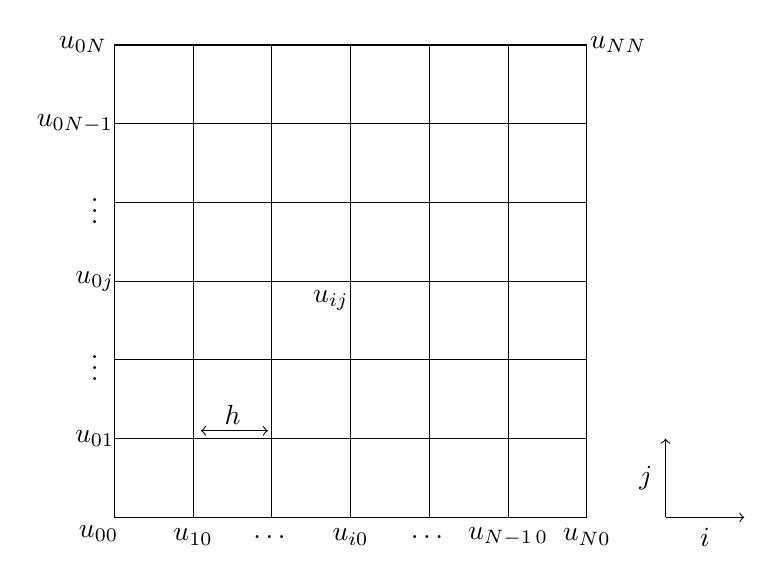
\begin{tikzpicture}
\draw (0,0) grid (6,6);
\node at (-0.2,-0.2) {$u_{00}$};
\node at (1,-0.25) {$u_{10}$};
\node at (2,-0.25) {$\dots$};
\node at (3,-0.25) {$u_{i0}$};
\node at (4,-0.25) {$\dots$};
\node at (5,-0.25) {$u_{N-1\,0}$};
\node at (6,-0.25) {$u_{N0}$};

\node at (-0.25,1) {$u_{01}$};
\node at (-0.25,2) {$\vdots$};
\node at (-0.25,3) {$u_{0j}$};
\node at (-0.25,4) {$\vdots$};
\node at (-0.5,5) {$u_{0N-1}$};
\node at (-0.4,6) {$u_{0N}$};

\node at (2.75,2.75) {$u_{ij}$};
\node at (6.4,6) {$u_{NN}$};

\draw[->] (7,0) -- (8,0);
\draw[->] (7,0) -- (7,1);
\node at (7.5,-0.25) {$i$};
\node at (6.75,0.5) {$j$};

\draw[<->] (1.1,1.1) -- (1.95,1.1);
\node at (1.5,1.3) {$h$};

\end{tikzpicture}
\centering
\caption{Discretised domain for $-u_{xx}-u_{yy}=f$.}
\end{figure}

The discretised form of this PDE can then be solved by computing the equation:
	\begin{equation}
	f_{ij} = -\frac{1}{h^2} \big( u_{i-1j} - 2u_{ij} + u_{i+1j} \big) - \frac{1}{h^2} \big( u_{ij-1} - 2u_{ij} + u_{ij+1} \big)
	\end{equation}
at each internal grid point, meaning the system has $n^2$ unknowns with $n=N-2$. 

The traditional approach to solving this discretised form would be to write (1.4) as:
	\begin{equation}
	f_{ij} = -\frac{1}{h^2} \big( u_{i-1j} + u_{ij-1} - 4u_{ij} + u_{i+1j} + u_{ij+1}  \big)
	\end{equation}
and then stack all unknowns $u_{ij}$ into a single vector $U$, resulting in the linear system $AU=F$. As stated previously, this ignores the underlying structure of the problem.

\subsection{Sylvester Equation}
A Sylvester equation is a matrix equation of the form $AX + XB = C$, where $A$ is a $n \times n$ matrix, $B$ is a $m \times m$ matrix, and $X$ and $C$ are $n \times m$ matrices. We can write (1.4) as a Sylvester equation in the form:
	\begin{equation}
	TU + UT = F
	\end{equation}
where $T$, $U$ and $F$ are of size $n \times n$.

Define $\text{tridiag}(i,j,k)$ as a matrix with $j$ on the main diagonal and $i$ and $k$ on the left and right diagonals respectively. Then for (1.6) we have $T=-\frac{1}{h^2} \, \text{tridiag}(1,-2,1)$ and $U_{ij} = u(x_i, y_j)$, where $(x_i, y_j)$ are interior grid nodes for $i,j=1,\dots,n$. The system has $n$ unknowns in each direction meaning there is a total of $n^2$ unknowns. The matrix equation is visualised below:
\begin{eqnarray}
\frac{-1}{h^2} 
\begin{pmatrix}
-2 & 1 & 0 & \dots & 0 & 0 \\
1 & -2 & 1 & \dots & 0 & 0 \\
0 & 1 & -2 & \dots & 0 & 0 \\
\vdots & \vdots & \vdots & \ddots & \vdots & \vdots \\
0 & 0 & 0 & \dots & -2 & 1 \\
0 & 0 & 0 & \dots & 1 & -2 \\
\end{pmatrix}
\begin{pmatrix}
u_{11} & u_{12} & \dots & u_{1j} & \dots & u_{1n} \\
u_{21} & u_{22} & \dots & u_{2j} & \dots & u_{2n} \\
\vdots & \vdots & \ddots & \vdots & \dots & \vdots \\
u_{i1} & u_{i2} & \dots & u_{ij} & \dots & u_{in} \\
\vdots & \vdots & \vdots & \vdots & \ddots & \vdots \\
u_{n1} & u_{n2} & \dots & u_{nj} & \dots & u_{nn}
\end{pmatrix} \nonumber \\ \nonumber
+
\begin{pmatrix}
u_{11} & u_{12} & \dots & u_{1j} & \dots & u_{1n} \\
u_{21} & u_{22} & \dots & u_{2j} & \dots & u_{2n} \\
\vdots & \vdots & \ddots & \vdots & \dots & \vdots \\
u_{i1} & u_{i2} & \dots & u_{ij} & \dots & u_{in} \\
\vdots & \vdots & \vdots & \vdots & \ddots & \vdots \\
u_{n1} & u_{n2} & \dots & u_{nj} & \dots & u_{nn}
\end{pmatrix}
\frac{-1}{h^2} 
\begin{pmatrix}
-2 & 1 & 0 & \dots & 0 & 0 \\
1 & -2 & 1 & \dots & 0 & 0 \\
0 & 1 & -2 & \dots & 0 & 0 \\
\vdots & \vdots & \vdots & \ddots & \vdots & \vdots \\
0 & 0 & 0 & \dots & -2 & 1 \\
0 & 0 & 0 & \dots & 1 & -2 \\
\end{pmatrix}
= F
\end{eqnarray}
There are a variety of methods that can be used to solve Sylvester equations. This project will explore and compare different methods for solving equations in this form. 

\subsection{Notation and Preliminaries}

\subsection{Organisation}

\newpage

\section{Scope and Schedule}
\subsection{Aim}
The aim of this project is to first study, implement and compare a range of matrix equation solvers. Following this, a specific problem will be derived with the help of my supervisor so that these solvers may be used and compared for a suitable application.

\subsection{Objectives}
The objectives of this project are as follows:
\begin{itemize}
\item To carry out an extensive, in-depth literature review on methods (both direct and iterative) for solving matrix equations from a wide range of sources. To decide which of these methods are appropriate to implement and to gain a solid understanding of how they work. 
\item To use and expand upon my programming experience to implement the chosen methods for solving matrix equations to solve the specified problem. 
\item To evaluate the implementation by comparing and contrasting the methods implemented to try to decide which is the best method for solving the given problem.
\item To derive a suitable application equation so that the methods studied in this project can be applied to a specific problem. 
\item To clearly present the work carried out during the project by using and building upon my report writing skills.
\end{itemize}

\subsection{Deliverables}
The deliverables of this project include:
\begin{itemize}
\item The final report that will include the details of the matrix solvers that have been studied, how the solvers were implemented, an evaluation and comparison of the implemented solvers, an analysis of how these solvers were used to solve the chosen application problem, and finally an evaluation of the success of the project.  
\item Code that successfully implements the chosen matrix solvers so that they solve the given problem.
\end{itemize}

\subsection{Methodology}
The methodology of this project will first involve studying academic publishings to gain an understanding of various methods for solving matrix equations. Python will be used as the programming language of choice for the implementation because of my familiarity with it, the extensive amount of documentation available for it and the excellent libraries it has available (e.g. NumPy and SciPy). GitHub will be used for version control and the final report will be written using \LaTeX. 

\subsection{Tasks, Milestones and Timeline}
The steps of this project will be divided into iterations, with the problem in each iteration becoming successively more complex and difficult to solve. This is because understanding is a key part of this project, and so each iteration will build on the understanding of the last. Each iteration will consist of studying and applying matrix methods to the problem, implementing them in Python to solve the problem, evaluating the results and write up. Also rough deadlines will be given for when each iteration should be completed by, to ensure the project is on track at any given stage.

The iterations are as follows:
\begin{itemize}
\item Introductory problem: $-u_{xx} - u_{yy} = 2 \pi^2 \sin{(\pi x)} \sin{(\pi y)}$ - deadline June 1st
\item Problem introducing uncertainty: $-\varepsilon u_{xx} - \varepsilon u_{yy} = 2 \pi^2 \sin{(\pi x)} \sin{(\pi y)}$ - deadline June 22nd
\item A Poisson equation on a surface defined by a height map (not yet derived) - deadline July 13th
\item Application reaction-diffusion equation (not yet derived) - deadline August 3rd
\end{itemize}

If the project deadlines are met the remaining time will be dedicated to project evaluation, write up and any possible project extensions.

\newpage

\section{Matrix Solvers}
For spatial domain $\mathcal{D} = \{(x,y) : 0 \leq x \leq 1, \; 0 \leq y \leq 1 \}$ and $u: \mathcal{D} \rightarrow \mathbb{R}$, let $u(x,y) = \sin{(\pi x)} \sin{(\pi y)}$ be the exact solution of the equation:
\begin{alignat}{2}
-u_{xx} -u_{yy} = {} & f \quad & \text{ on } \mathcal{D} \nonumber \\
u = {} & 0 \quad & \text{ on } \partial \mathcal{D}
\end{alignat}

This gives:
\begin{equation}
\begin{split}
u_{xx} = u_{yy} = - \pi^2 \sin{(\pi x)} \sin{(\pi y)} \\
\implies f = 2 \pi^2 \sin{(\pi x)} \sin {(\pi y)}
\end{split}
\end{equation} 

The equation to be be solved is therefore:
\begin{alignat}{1}
-u_{xx} -u_{yy} = {} & 2 \pi^2 \sin{(\pi x)} \sin {(\pi y)} \quad \text{ on } \mathcal{D} \nonumber \\
u = {} & 0 \quad \text{ on } \partial \mathcal{D}
\end{alignat}

Using the centred finite difference approximations ((1.2) and (1.3)) with uniform grid spacing $h$ to discretise the domain of this system, we have:
	\begin{equation}
	\begin{split}
	-\frac{1}{h^2} \big( u_{i-1j} - & 2u_{ij} + u_{i+1j} \big) - \frac{1}{h^2} \big( u_{ij-1} - 2u_{ij} + u_{ij+1} \big) 
	\\ & = 2\pi^2 \sin(\pi x_i) \sin(\pi y_j)
	\end{split}
	\end{equation}
to be solved at each grid point for $i, j = 1, \dots n$, where $n$ is the total number of unknowns in each direction. The matrix form of this equation is therefore:
\begin{equation}
	TU + UT = F
	\end{equation}
where $T=-\frac{1}{h^2} \, \text{tridiag}(1,-2,1)$, $U_{ij} = u(x_i, y_j)$ and $F_{ij} = 2 \pi^2 \sin(\pi x_i) \sin(\pi y_j)$ are all matrices of size $n \times n$ and $(x_i, y_j)$ are interior grid nodes for $i,j=1,\dots,n$.

This form allows us to explore different methods for solving this equation and compare them to the exact solution $u = \sin(\pi x) \sin(\pi y)$. A plot of the exact solution, with $n=1000$, is given in Figure 3. 

\begin{figure}[H]
\includegraphics[scale=.5]{img/solution2.png}
\centering
\caption{Plot of the solution with $n=1000$.}
\end{figure} 

Throughout the following section, the following measurements are given to evaluate the performance of each of the methods implemented:
\begin{itemize}
\item $n$: The number of unknowns in each direction for the system. The total number of unknowns is $n^2$.
\item Time(s): The time taken in seconds for the method to compute the solution to the problem.
\item $|| u - u_h ||_{L^\infty} $: Measures the maximum difference between the actual solution and computed solution for each $u$. Defined as:
 \[ || u - u_h ||_{L^\infty} = \text{max}_{ij} | u(x_i, y_i) - u_{ij} | \]
\item $|| u - u_h ||_{L^2} $: An average measure of error, defined as:
\[ || u - u_h ||_{L^2} = \sqrt{h^2 \sum | u(x_i,y_j) - u_{ij} |^2} \]
\item Experimental order of convergence (eoc): Measures the rate of convergence of a method as the problem size is increased, which should approach 2 as the step size is increased. Defined as:
\[ \text{eoc}(i) = \frac{\log(\nicefrac{E_i}{E_{i-1}})}{\log(\nicefrac{h_i}{h_{i-1}})} \]
where $E_i$ is the error (chosen here as $|| u - u_h ||_{L^\infty}$) and $h_i$ is the mesh size at level $i$. 
\item Experimental order of growth (eog): Measures the order of growth of the execution time of an algorithm as the problem size is increased (that is, the approximate time complexity). Defined as:
\[ \text{eog}(i) = \frac{\log(\nicefrac{t_{i}}{t_{i-1}})}{\log(\nicefrac{n_{i}}{n_{i-1}})} \]
where $t_i$ is the total execution time and $n_i$ is the problem size at level $i$.
\item No. iters (iterative methods only): The number of iterations taken for the method to converge to the given convergence tolerance.
\end{itemize}
It is worth noting that as the total number of unknowns, and therefore the problem size, is $n^2$, the best time complexity that an optimal solver can achieve is $O(n^2)$, as it must compute a solution for each unknown. 

For each of the implemented methods, a maximum running time of 6000 seconds will be given. If a method does not compute a solution in this time, this will be specified in the results. If a method does not compute a solution because it tries to use more memory than is available, this will also be specified in the results.

\subsection{Direct Methods}

\subsubsection{Kronecker Product}
A naive approach to solving this system is to use the Kronecker product to rewrite (3.5) as a standard vector linear system. The Sylvester equation $AX + XB = C$ can be written as the standard vector linear system:
\begin{equation}
\mathcal{A}x = c
\end{equation}
with $\mathcal{A} = I \otimes A + B^* \otimes I$, where $I$ is the identity matrix, $B^*$ denotes the conjugate transpose of $B$, $x = \text{vec}(X)$ and $c = \text{vec}(C)$.\footnote{The vec operator reshapes a matrix into a vector by stacking the columns one after another.}

The equivalent linear system for the matrix equation $TU + UT = F$ is:
\begin{equation}
\mathcal{T}u = \mathcal{F}
\end{equation}
where $\mathcal{F} = \text{vec}(F)$, $\mathcal{T} = I \otimes T + T \otimes I$ and $u = \text{vec}(U)$. 

This is the exact linear system that would be obtained from equation (1.5), i.e. stacking all unknowns $u_{ij}$ into a single vector in the first place. Since the matrix $\mathcal{T}$ is sparse, this equation can be solved using a standard direct sparse solver. This approach provides a good base case for comparison. Results solving this linear system using the direct sparse solver \texttt{sparse.linalg.spsolve} from the SciPy library are shown in Table 1. As can be seen from the results, both errors decrease as the problem size $n$ is increased. The eoc is very close to 2 for all $n$, demonstrating the convergence of the algorithm. As $n$ is increased the eog grows beyond $3$, which shows this algorithm has worse than cubic time complexity for large $n$. 

\begin{table}[H]
\centering
\begin{tabular}{|c|c|c|c|c|c|}
\hline
$n$ & Time(s) & $|| u - u_h ||_{L^{\infty}}$ &$|| u - u_h ||_{L^{2}}$ & eoc & eog \\
\hline
125 & 0.18141 & $5.1807 \times 10^{-5}$ & $2.5904 \times 10^{-5}$ & - & - \\
250 & 0.60371 & $1.3054 \times 10^{-5}$ & $6.5275 \times 10^{-6}$ & 2.0001 & 1.7346 \\
500 & 4.1663 & $3.2767 \times 10^{-6}$ & $1.6384 \times 10^{-6}$ & 1.9999 & 2.7868 \\
1000 & 36.113 & $8.2082 \times 10^{-7}$ & $4.1041 \times 10^{-7}$ & 2.0000 & 3.1157 \\
2000 & 404.48 & $2.0539 \times 10^{-7}$ & $1.0267 \times 10^{-7}$ & 2.0001 & 3.4855 \\
\cline{2-6}
4000 & \multicolumn{5}{c|}{Memory Error} \\
\hline
\end{tabular}
\captionsetup{justification=centering}
\caption{Results obtained from solving the linear system $\mathcal{A} x = c$ using the direct solver  \texttt{sparse.linalg.spsolve} from the SciPy library.}
\end{table}

\subsubsection{Bartels-Stewart Algorithm}
The Bartels-Stewart algorithm \cite{Bartels} can be used to solve the Sylvester equation $AX + XB = C$. 
This algorithm works by computing the Schur decompositions of the coefficient matrices $A$ and $B$, which are used to transform the equation into an equivalent form which is triangular, meaning it can be solved one element at a time. The solution of this triangular system is then used to obtain the solution to the original equation.

In the general case the algorithm is as follows:
\begin{enumerate}
\item Compute the Schur forms $A^* = PRP^*$ and $B=QSQ^*$
\item Solve $R^*V + VS = P^*CQ$ for $V$
\item Compute $X=PVQ^*$
\end{enumerate}
where $A^*$ denotes the conjugate transpose of $A$.

For the equation $TU+UT=F$, the algorithm is as follows:
\begin{enumerate}
\item Compute the Schur form $T=PRP^*$
\item Solve $R^*V + VR = P^*FP$ for $V$
\item Compute $U=PVP^*$
\end{enumerate}

Results using this algorithm are shown in Table 2. These results show that both errors decrease as $n$ is increased. Also the eoc is close enough to 2 to conclude that this algorithm converges. The eog demonstrates that this algorithm has an approximate cubic time complexity. 

\begin{table}[H]
\centering
\begin{tabular}{|c|c|c|c|c|c|}
\hline
$n$ & Time(s) & $|| u - u_h ||_{L^{\infty}}$ &$|| u - u_h ||_{L^{2}}$ & eoc & eog \\
\hline
125 & 1.2486 & $5.1807 \times 10^{-5}$ & $2.5904 \times 10^{-5}$ & - & - \\
250 & 9.6712 & $1.3054 \times 10^{-5}$ & $6.5275 \times 10^{-6}$ & 2.0001 & 2.9124 \\
500 & 77.888 & $3.2767 \times 10^{-6}$ & $1.6384 \times 10^{-6}$ & 1.9999 & 3.0096 \\ 
1000 & 640.22 & $8.2088 \times 10^{-7}$ & $4.1044 \times 10^{-7}$ & 2.0000 & 3.0391 \\
2000 & 5093.1 & $2.0467 \times 10^{-7}$ & $1.0237 \times 10^{-7}$ & 2.0052 & 2.9919 \\
\cline{2-6}
4000 & \multicolumn{5}{c|}{Timing Error} \\
\hline
\end{tabular}
\caption{Results using the Bartels-Stewart algorithm.}
\end{table}

By breaking this algorithm down into its component parts, we can time each step to see which is the most costly. The results of doing so are given in Table 3, where the steps are:

\begin{enumerate}
\item Compute the Schur form $T=PRP^*$ (using \texttt{linalg.schur} from the SciPy library)
\item Solve the $R^*V + VR = P^*FP$ for $V$, which is a triangular system
\item Compute the solution $U=PVP^*$
\end{enumerate}

As can be seen from the results in Table 3, the most costly part of the algorithm is by far the second step, which is due to the fact that solving the triangular system uses back substitution which requires multiple nested \texttt{for} loops.

\begin{table}[H]
\centering
\begin{tabular}{|c|c|c|c|c|}
\hline
$n$ & 1 & 2 & 3 & Total \\
\hline
125 & 0.012667 & 1.2357 & 0.00023031 & 1.2486 \\
250 & 0.048434 & 9.6218 & 0.0010102 & 9.6712 \\
500 & 0.26262 & 77.619 & 0.0064600 & 77.888 \\ 
1000 & 0.083478 & 639.34 & 0.043818 & 640.22 \\
2000 & 5.1290 & 5087.5 & 0.41275 & 5093.1 \\
\hline
\end{tabular}
\caption{Timings for each step using the Bartels-Stewart algorithm.}
\end{table}

The SciPy library has a built in solver for solving Sylvester equations, \texttt{linalg.solve \_sylvester}, which uses the Bartels-Stewart algorithm. Results using this solver are given in Table 4. The errors here are similar to the errors given in Table 2. Again the eoc is close enough to 2 to conclude that this algorithm converges. However, the eog seems to vary depending on the problem size $n$. 

\begin{table}[H]
\centering
\begin{tabular}{|c|c|c|c|c|c|}
\hline
$n$ & Time(s) & $|| u - u_h ||_{L^{\infty}}$ &$|| u - u_h ||_{L^{2}}$ & eoc & eog \\
\hline
125 & 0.059959 & $5.1807 \times 10^{-5}$ & $2.5904 \times 10^{-5}$ & - & - \\
250 & 0.11421 & $1.3054 \times 10^{-5}$ & $6.5275 \times 10^{-6}$ & 2.0001 & 0.92964 \\
500 & 1.9383 & $3.2767 \times 10^{-6}$ & $1.6384 \times 10^{-6}$ & 1.9999 & 4.0850  \\
1000 & 4.0920 & $8.2084 \times 10^{-7}$ & $4.1042 \times 10^{-7}$ & 2.0000 & 1.0780 \\
2000 & 32.029 & $2.0503 \times 10^{-7}$ & $1.0259 \times 10^{-7}$ & 2.0027 & 2.9685  \\
4000 & 279.95 & $4.9949 \times 10^{-8}$ & $2.4876 \times 10^{-8}$ & 2.0377 & 3.1277  \\
8000 & 2812.2 & $8.6380 \times 10^{-9}$ & $4.1216 \times 10^{-9}$ & & \\
\cline{2-6}
16000 & \multicolumn{5}{c|}{Timing error} \\
\hline
\end{tabular}
\caption{Results using SciPy's \texttt{linalg.solve\_sylvester}.}
\end{table}

As can be seen from the results above, using the built-in SciPy solver results in a significant speed-up in time as $n$ is increased. This is likely because it makes use of of LAPACK, which is an optimised software library for solving linear algebra problems.


\subsubsection{Similarity Transformation}
A similarity transformation \cite{Simoncini} can be used to solve the Sylvester equation $AX + XB = C$. This method uses an eigendecomposition to rewrite the equation into a form that the solution can be easily obtained from. The method is as follows.

Assuming matrices $A$ and $B$ can be diagonalised, let $P^{-1}AP = \text{diag}(\lambda_1, \dots, \lambda_n)$ and $Q^{-1}BQ = \text{diag}(\mu_1, \dots, \mu_m)$, where $\lambda_1, \dots, \lambda_n$ are the eigenvalues of $A$, $\mu_1, \dots, \mu_m$ are the eigenvalues values of $B$ and the columns of $P$ and $Q$ are the eigenvectors of $A$ and $B$, respectively. Letting $\widetilde{C} = P^{-1}CQ$, the solution is then:
\[ X = P \widetilde{X} Q^{-1}, \text{ with } \widetilde{X}_{ij} = \frac{\widetilde{C}_{ij}}{\lambda_i + \mu_j} \]

For $TU+UT=F$, we have $P=Q$ and $P^{-1}TP = \text{diag}(\lambda_1, \dots, \lambda_n)$, where $\lambda_1, \dots, \lambda_n$ are the eigenvalues of $T$ and the columns of $P$ are the eigenvectors of $T$. Letting $\widetilde{F}=P^{-1}FP$, the solution is then:
\[ U = P \widetilde{U} P^{-1}, \text{ with } \widetilde{U}_{ij} = \frac{\widetilde{F}_{ij}}{\lambda_i + \lambda_j} \]

\subsubsection*{Using numpy.linalg.eig}
Using the method above, the eigenvalues and eigenvectors can be computed using NumPy's \texttt{linalg.eig} function. The results doing this are given in Table 5. The errors are again similar to the previous methods. However, here the eoc moves away from 2 as $n$ is increased. This is likely due to the fact that there is no general formula for calculating eigenvalues and eigenvectors for an arbitrary matrix, meaning the eigenvalues and eigenvectors are most likely approximated by NumPy's \texttt{linalg.eig}. It is likely that the approximations become less accurate as $n$ is increased. The eog here is however slightly better than the previous methods. 

\begin{table}[H]
\centering
\begin{tabular}{|c|c|c|c|c|c|}
\hline
$n$ & Time(s) & $|| u - u_h ||_{L^{\infty}}$ &$|| u - u_h ||_{L^{2}}$ & eoc & eog \\
\hline
125 & 0.034534 & $5.1802 \times 10^{-5}$ & $2.5904 \times 10^{-5}$ & -  & - \\
250 & 0.13690 & $1.3054 \times 10^{-5}$ & $6.5275 \times 10^{-6}$ & 2.0000 & 1.9870  \\
500 & 0.59718 & $3.2767 \times 10^{-6}$ & $1.6384 \times 10^{-6}$ & 1.9999 & 2.1250  \\
1000 & 2.2211 & $8.2086 \times 10^{-7}$ & $4.1043 \times 10^{-7}$ & 1.9999 & 1.8950  \\
2000 & 11.571 & $2.0467 \times 10^{-7}$ & $1.0237 \times 10^{-7}$ & 2.0053 & 2.3812  \\
4000 & 70.984 & $4.9966 \times 10^{-8}$ & $2.4876 \times 10^{-8}$ & 2.0350 & 2.6170  \\
8000 & 466.83 & $8.6360 \times 10^{-9}$ & $4.1223 \times 10^{-9}$ & 2.5330 & 2.7173  \\
\cline{2-6}
16000 & \multicolumn{5}{c|}{Memory Error} \\
\hline
\end{tabular}
\captionsetup{justification=centering}
\caption{Results using a similarity transformation, calculating the eigenvalues and eigenvectors using \texttt{numpy.linalg.eig}.}
\end{table}

Similarly to the Bartels-Stewart algorithm, this method can be split into component parts and each part can be timed, to see which part is the most costly. The steps of the method are:
\begin{enumerate}
\item Calculate eigenvalues and eigenvectors of $T$
\item Diagonalise $T$ (i.e. calculate $P$ and $P^{-1}$)
\item Calculate $\widetilde{F}=P^{-1}FP$
\item Calculate $\widetilde{U}$, where $\widetilde{u}_{ij} = \frac{\widetilde{f}_{ij}}{\lambda_i + \lambda_j}$
\item Calculate solution $U=P \widetilde{U}P^{-1}$
\end{enumerate}

The results of doing so are shown in Table 6.

\begin{table}[H]
\centering
\begin{tabular}{|c|c|c|c|c|c|c|}
\hline
$n$ & 1 & 2 & 3 & 4 & 5 & Total \\
\hline
125 & 0.013860 & 0.00042105 & 0.00075817 & 0.018881 & 0.00061440 & 0.034534 \\
250 & 0.052402 & 0.00068998 & 0.0026329 & 0.078654 & 0.0025253 & 0.13690 \\
500 & 0.25900 & 0.0020170 & 0.013870 & 0.30815 & 0.014147 & 0.59718 \\
1000 & 0.91819 & 0.0011129 & 0.084650 & 1.1328 & 0.084323 & 2.2211 \\
2000 & 5.8236 & 0.0035102 & 0.61534 & 4.5150 & 0.61360 & 11.571 \\
4000 & 43.651 & 0.0074658 & 4.6290 & 18.071 & 4.6257 & 70.984 \\
8000 & 325.30 & 0.027416 & 35.464 & 70.695 & 35.345 & 466.83 \\
\hline
\end{tabular}
\captionsetup{justification=centering}
\caption{Timing results for each step of the similarity transformation method, calculating the eigenvalues and eigenvectors using \texttt{numpy.linalg.eig}.}
\end{table}

\subsubsection*{Calculating eigenvalues and eigenvectors explicitly}

As can be seen from the results in Table 6, the most costly part of this method is calculating the eigenvalues and eigenvectors. As $T$ is a matrix in Toeplitz form, we can instead compute the eigenvalues and eigenvectors directly as:
\begin{equation} 
\lambda_i = \frac{2}{h^2} \Big( \cos \Big( \frac{i \pi}{n+1} \Big) - 1 \Big) 
\end{equation}
and:
\begin{equation}
t_{ij} = \sqrt{\frac{2}{n+1}} \sin \Big( \frac{ij \pi}{n+1}  \Big) 
\end{equation}

Also the matrix $P$ is Hermitian, which means that $P^{-1} = P^T$. We can use both of these properties to improve the timings of this algorithm. Results of doing so are given in Table 7, and timings for each step are given in Table 8. 

%Similar errors are given by this method, however the eoc is  closer to 2 for $n \leq 8000$. When $n=16000$ the eoc increases significantly, however the errors here are so small that this is likely due to the impact of roundoff errors. The eog is also significantly less demonstrating that using this algorithm and computing the eigenvalues explicity achieves a near square time complexity. Also this is the only method so far that has been able to solve the problem with $n=16000$ without running out of memory. 

\begin{table}[H]
\centering
\begin{tabular}{|c|c|c|c|c|c|}
\hline
$n$ & Time(s) & $|| u - u_h ||_{L^{\infty}}$ &$|| u - u_h ||_{L^{2}}$ & eoc & eog\\
\hline
125 & 0.028324 & $5.1807 \times 10^{-5}$ & $2.5904 \times 10^{-5}$ & - & -  \\
250 & 0.080759 & $1.3054 \times 10^{-5}$ & $6.5275 \times 10^{-6}$ &  &   \\
500 & 0.22574 & $3.2767 \times 10^{-6}$ & $1.6384 \times 10^{-6}$ &  &  \\
1000 & 0.87985 & $8.2082 \times 10^{-7}$ & $4.1041 \times 10^{-7}$ &  &   \\
2000 & 4.0533 & $2.0541 \times 10^{-7}$ & $1.0270 \times 10^{-7}$ &  &  \\
4000 & 15.696 & $5.1313 \times 10^{-8}$ & $2.5656 \times 10^{-8}$ &  &   \\
8000 & 73.321 & $1.2813 \times 10^{-8}$ & $6.4065 \times 10^{-9}$ &  &   \\
16000 & 428.46 & $7.7527 \times 10^{-10}$ & $3.8764 \times 10^{-10}$ &  &  \\
\cline{2-6}
32000 & \multicolumn{5}{c|}{Memory Error??} \\
\hline
\end{tabular}
\captionsetup{justification=centering}
\caption{Results using a similarity transformation, calculating the eigenvalues and eigenvectors explicity.}
\end{table}

\begin{table}[H]
\centering
\begin{tabular}{|c|c|c|c|c|c|c|}
\hline
$n$ & 1 & 2 & 3 & 4 & 5 & Total \\
\hline
125 & 0.057252 & 0.00025916 & 0.0045545 & 0.018010 & 0.00059748 & 0.080673 \\
250 & 0.21954 & 0.00047016 & 0.0081279 & 0.073295 & 0.0025220 & 0.30396 \\ 
500 & 0.88125 & 0.0012608 & 0.018555 & 0.28724 & 0.013819 & 1.2021  \\
1000 & 3.7073 & 0.00096869 & 0.67056 & 1.1304 & 0.081200 & 5.5904 \\
2000 & 13.812 & 0.0092294 & 1.3690 & 4.4495 & 0.60793 & 20.247 \\
4000 & 54.907 & 0.0068946 & 4.9050 & 17.381 & 4.5936 & 82.243 \\
8000 & 217.26 & 0.026015 & 35.357 & 71.581 & 36.129 & 360.35 \\
16000 & 892.51 & 168.51 & 217.68 & 288.92 & 204.25 & 1771.9 \\
\hline
\end{tabular}
\captionsetup{justification=centering}
\caption{Timing results for each step of the similarity transformation method, calculating the eigenvalues and eigenvectors explicitly.}
\end{table}

As can be seen from the results in Table 8, calculating the eigenvalues and eigenvectors explicitly  outperforms calculating them using the NumPy library when $n$ is large.

\subsubsection{Shifted System}
A projection method \cite{Simoncini} can be used to solve $AX + XB = C$. This method works by computing the eigendecomposition of $B$ to reform the problem as solving $n$ independent linear systems. Each of these linear systems can be solved simultaneously to obtain the solution $X$. The steps of this method are as follows:
\begin{enumerate}
\item Compute $B = WSW^{-1}$, where $S = \text{diag}(s_1, \dots, s_n)$ are the eigenvalues of $B$ and the columns of $W$ are the eigenvectors of $B$
\item Compute $\hat{C} = CW$
\item For $i=1$ to $n$, solve the system $(A+s_i I)(\hat{X})_i = (\hat{C})_i$
\item Compute solution $X = \hat{X}W$
\end{enumerate}
where $(\hat{X})_i$ denotes the $i^{\text{th}}$ column of $\hat{X}$.

In the case of $TU + UT = F$, the steps are as follows:
\begin{enumerate}
\item Compute $T = WSW^{-1}$, where $S = \text{diag}(s_1, \dots, s_n)$ are the eigenvalues of $T$ and the columns of $W$ are the eigenvectors of $T$
\item Compute $\hat{F} = FW$
\item For $i=1$ to $n$, solve the system $(T+s_i I)(\hat{U})_i = (\hat{F})_i$
\item Compute solution $U = \hat{U}W$
\end{enumerate}

Results using this method are given in Table 9. The errors are approximately the same as the errors given previously. The eoc is approximately 2 and the eog is $> 3$ for large $n$ demonstrating that this algorithm converges with a worse than cubic time complexity. 
\begin{table}[H]
\centering
\begin{tabular}{|c|c|c|c|c|c|}
\hline
$n$ & Time(s) & $|| u - u_h ||_{L^{\infty}}$ &$|| u - u_h ||_{L^{2}}$ & eoc & eog \\
\hline
125 & 0.092085 & $5.1807 \times 10^{-5}$ & $2.5904 \times 10^{-5}$ & - & - \\
250 & 0.43609 & $1.3054 \times 10^{-5}$ & $6.5274 \times 10^{-6}$ & 2.0001 & 2.2436 \\
500 & 2.1851 & $3.2767 \times 10^{-6}$ & $1.6384 \times 10^{-6}$ & 1.9999 & 2.3250 \\
1000 & 19.498 & $8.2082 \times 10^{-7}$ & $4.1041 \times 10^{-7}$ & 2.0000 & 3.1576 \\
2000 & 194.13 & $2.0541 \times 10^{-7}$ & $1.0271 \times 10^{-7}$ & 2.0000 & 3.3156 \\
4000 & 2452.5 & $5.1347 \times 10^{-8}$ & $2.5674 \times 10^{-8}$ & 2.0009 & 3.6592  \\
\cline{2-6} 
8000 & \multicolumn{5}{c|}{Timing error} \\
\hline
\end{tabular}
\captionsetup{justification=centering}
\caption{Results using a projection method to solve $n$ linear systems.}
\end{table}

The steps of this method can also be broken down into component parts and each part timed. The results of doing so are given in Table 10. Unsuprisingly, the most costly part of the algorithm is solving the $n$ linear systems. 

\begin{table}[H]
\centering
\begin{tabular}{|c|c|c|c|c|c|}
\hline
$n$ & 1 & 2 & 3 & 4 & Total \\
\hline
125 & 0.057421 & 0.0043032 & 0.3028 & $7.1764 \times 10^{-7}$ & 0.092085 \\
250 & 0.23967 & 0.0041912 & 0.19177 & 0.00046206 & 0.43609  \\
500 & 0.85408 & 0.0079994 & 1.3200 & 0.0030336 & 2.1851 \\
1000 & 3.3709 & 0.026276 & 16.079 & 0.021675 & 19.498 \\
2000 & 13.278 & 0.50065 & 180.81 & 0.16621 & 194.13 \\
4000 & 53.300 & 1.8301 & 2396.1 & 1.2866 & 2452.5  \\
\hline
\end{tabular}
\captionsetup{justification=centering}
\caption{Timing results of each step using a projection method to solve $n$ linear systems.}
\end{table}

\subsection{Iterative Methods}

\subsubsection{Kronecker Product}
Similarly to Section 3.1.1, the Kronecker product can be used to write the matrix equation as a standard vector linear system. A a standard iterative solver can then be used to solve the system, which can provide a base case for comparison. Results using \texttt{scipy.sparse.linalg.cg}, which is a sparse solver that uses the conjugate gradient iterative method, are given in Table 11, using a convergence tolerance of $10^{-9}$. The results show errors similar to all the direct methods. The eoc demonstrates that the algorithm converges very well. Although this algorithm is much faster than all the previous direct methods, the eog demonstrates that when $n$ is significantly large, the algorithm exhibits a worse than cubic time complexity, which is shown here when $n=8000$.  

\begin{table}[H]
\centering
\begin{tabular}{|c|c|c|c|c|c|c|}
\hline
$n$ & Time(s) & no. iters & $|| u - u_h ||_{L^{\infty}}$ &$|| u - u_h ||_{L^{2}}$ & eoc & eog \\
\hline
125 & 0.014182 & 1 & $5.1807 \times 10^{-5}$ & $2.5904 \times 10^{-5}$ & - & - \\
250 & 0.042605 & 1 & $1.3054 \times 10^{-5}$ & $6.5275 \times 10^{-6}$ & 2.0001 & 1.5870 \\
500 & 0.14136 & 1 & $3.2767 \times 10^{-6}$ & $1.6384 \times 10^{-6}$ & 1.9999 & 1.7303 \\
1000 & 0.54308 & 1 & $8.2082 \times 10^{-7}$ & $4.1041 \times 10^{-7}$ & 2.0000 & 1.9418 \\
2000 & 2.3162 & 1 & $2.0541 \times 10^{-7}$ & $1.0271 \times 10^{-7}$ & 2.0000 & 2.0925 \\
4000 & 9.8487 & 1 & $5.1379 \times 10^{-8}$ & $2.5689 \times 10^{-8}$ & 2.0000 & 2.0882 \\
8000 & 103.34 & 2 & $1.2848 \times 10^{-8}$ & $6.4239 \times 10^{-9}$ & 2.0000 & 3.3913 \\
\cline{2-7}
16000 & \multicolumn{6}{c|}{Memory Error} \\
\hline
\end{tabular}
\captionsetup{justification=centering}
\caption{Results obtained from solving the linear system $\mathcal{A} x = c$ using the iterative solver  \texttt{sparse.linalg.cg} from the SciPy library.}
\end{table}

\subsubsection{Gradient Based Method}
In \cite{Zhou} a gradient based method for solving Sylvester equations is given. The equation $TU + UT = F$ can be written as two recursive sequences:
	\begin{equation}
	U_k^{(1)} = U_{k-1}^{(1)} + \kappa T(F-TU_{k-1}^{(1)} - U_{k-1}^{(1)}T)
	\end{equation}
	\begin{equation}
	U_k^{(2)} = U_{k-1}^{(2)} + \kappa (F-TU_{k-1}^{(2)} - U_{k-1}^{(2)}T)T
	\end{equation}
where $\kappa$ represents the relative step size. The approximate solution $U_k$ is taken as the average of these two sequences:
	\begin{equation}
	U_k = \frac{U_k^{(1)} + U_k^{(2)}}{2}
	\end{equation}
This solution only converges if:
	\begin{equation}
	0 < \kappa < \frac{1}{\lambda_{\text{max}}(T^2)} 
	\end{equation}
where $\lambda_{\text{max}}(T^2)$ denotes the maximum eigenvalue of $T^2$. We can use the formula (3.8) to calculate the maximum eigenvalue of $T^2$ as:
\begin{equation}
\lambda_{\text{max}}(T^2) = \frac{4}{h^4} \text{max} \Big( \big( \cos{\Big(\frac{i \pi}{n+1} \Big) } -1 \big)^2 \Big)
\end{equation}
$\lambda_{\text{max}}(T^2)$ therefore scales with $\frac{1}{h^4}$ meaning its reciprocal scales with $h^4$. This implies that $\kappa$ will need to be significantly small as $n$ is increased for the solution to converge. Even for small values of $n$, this is impractical and therefore this method is not appropriate for solving this equation. This can be seen from the fact that, using this method with $n=125$ and a step size of $\kappa = \nicefrac{1}{2 \lambda_{\text{max}}(T^2)}$, the method took longer than the maximum time of 6000 seconds allowed to compute a solution.

\subsubsection{Modified Conjugate Gradient}
In \cite{Hou} a modified conjugate gradient (MCG) algorithm is proposed, which is adapted for solving Sylvester Equations. The general algorithm for solving $AX+XB=C$, where $A, B, C$ and $X$ are all $n \times n$ matrices, is as follows:
\begin{enumerate}
\item Choose initial guess $X^{(0)}$ and calculate:
	\begin{itemize}
	\item $R^{(0)} = C - AX^{(0)} - X^{(0)}B$
	\item $Q^{(0)} = A^T R^{(0)} + R^{(0)} + R^{(0)} B^T$
	\item $Z^{(0)} = Q^{(0)}$
	\end{itemize}
\item If $R^{(k)} < \text{tol}$ or $Z^{(k)} < \text{tol}$, stop. Else, go to 3.
\item Calculate:
	\begin{itemize}
	\item $\gamma_k = \frac{[R^{(k)}, R^{(k)}]}{[Z^{(k)}, Z^{(k)}]}$, where $[R,R] = \text{tr}(R^T R)$ is the trace of the matrix $R^T R$
	\item $X^{(k+1)} = X^{(k)} + \gamma_k Z^{(k)}$
	\item $R^{(k+1)} = C - AX^{(k+1)} - X^{(k+1)} B$
	\item $Q^{(k+1)} = A^T R^{(k+1)} + R^{(k+1)} + R^{(k+1)} B^T$
	\end{itemize}
	and return to Step 2.
\end{enumerate}

In the case of the matrix equation $TU+UT=F$, the algorithm is as follows:
\begin{enumerate}
\item Choose initial guess $U^{(0)}$ and calculate:
	\begin{itemize}
	\item $R^{(0)} = F - TU^{(0)} - U^{(0)}T$
	\item $Q^{(0)} = T R^{(0)} + R^{(0)} + R^{(0)} T$
	\item $Z^{(0)} = Q^{(0)}$
	\end{itemize}
\item If $R^{(k)} < \text{tol}$ or $Z^{(k)} < \text{tol}$, stop. Else, go to 3.
\item Calculate:
	\begin{itemize}
	\item $\gamma_k = \frac{[R^{(k)}, R^{(k)}]}{[Z^{(k)}, Z^{(k)}]}$
	\item $U^{(k+1)} = U^{(k)} + \gamma_k Z^{(k)}$
	\item $R^{(k+1)} = F - TU^{(k+1)} - U^{(k+1)} T$
	\item $Q^{(k+1)} = T R^{(k+1)} + R^{(k+1)} + R^{(k+1)} T$
	\end{itemize}
	and return to Step 2.
\end{enumerate}

Results using this algorithm with a convergence tolerance of $10^{-3}$ are given in Table 12. These results show that, even when using this relatively large convergence tolerance, this algorithm is slow. Also the errors does not always decrease as $n$ is increased, which is reflected in the eoc. The errors here are also bigger than those for previous methods for large $n$, which is due to the large convergence tolerance. The eog demonstrates that this algorithm has a worse than cubic time complexity for large $n$.

\begin{table}[H]
\centering
\begin{tabular}{|c|c|c|c|c|c|}
\hline
$n$ & Time(s) & $|| u - u_h ||_{L^{\infty}}$ &$|| u - u_h ||_{L^{2}}$ & eoc & eog \\
\hline
125 & 11.006 & $1.1451 \times 10^{-6}$ & $5.7254 \times 10^{-7}$ & - & - \\
250 & 53.234 & $3.7599 \times 10^{-5}$ & $1.8800 \times 10^{-5}$ & -5.0662 & 2.2741 \\
500 & 397.11 & $4.6673 \times 10^{-5}$ & $2.3337 \times 10^{-5}$ & -0.31294 & 2.8991 \\
1000 & 3865.5 & $3.3353 \times 10^{-5}$ & $1.6677 \times 10^{-5}$ & 0.48547 & 3.2830 \\
\hline
\end{tabular}
\captionsetup{justification=centering}
\caption{Results obtained using the MCG algorithm.}
\end{table}

\subsubsection{Preconditioned MCG}
\cite{Hou} also proposes a preconditioned version of the MCG algorithm which accelerates the speed of convergence. This version of the algorithm solves $AX + XB = C$ by solving the equation 
$X^{(k+1)} = \widetilde{A}X^{(k)} \widetilde{B} + \widetilde{C}$, with:
\[ \widetilde{A} = I + 2(\alpha A - I)^{-1} \]
\[ \widetilde{B} = I + 2(\alpha B - I)^{-1} \]
\[ \widetilde{C} = -2\alpha(\alpha A - I)^{-1} C (\alpha B - I)^{-1} \]
where $\alpha$ is a parameter that needs to be chosen and $I$ is the identity matrix. \cite{Hou} suggests choosing $\alpha = \pm \nicefrac{\sqrt{n}}{||A||_F}$ or $\alpha = \pm \nicefrac{\sqrt{n}}{||B||_F}$, where $||A||_F = \sqrt{[A,A]} = \sqrt{\text{tr}(A^TA)}$, for good convergence. Once $\alpha$ has been chosen and $\widetilde{A}, \widetilde{B}$ and $\widetilde{C}$ have been calculated, the algorithm is as follows:
\begin{enumerate}
\item Choose initial guess $X^{(0)}$ and calculate:
	\begin{itemize}
	\item $R^{(0)} = -\widetilde{C} + X^{(0)} - \widetilde{A}X^{(0)} \widetilde{B}$
	\item $Q^{(0)} = \widetilde{A}^T R^{(0)}\widetilde{B}^T + R^{(0)}$
	\item $Z^{(0)} = Q^{(0)}$
	\end{itemize}
\item If $R^{(k)} < \text{tol}$ or $Z^{(k)} < \text{tol}$, stop. Else, go to 3.
\item Calculate:
	\begin{itemize}
	\item $ \gamma_k = \frac{[R^{(k)}, R^{(k)}]}{[Z^{(k)}, Z^{(k)}]}$
	\item $X^{(k+1)} = X^{(k)} + \gamma_k Z^{(k)} $
	\item $R^{(k+1)} = -\widetilde{C} + X^{(k+1)} - \widetilde{A}X^{(k+1)} \widetilde{B}$
	\item $Q^{(k+1)} = \widetilde{A}^T R^{(k+1)}\widetilde{B}^T - R^{(k+1)}$
	\item $\eta_k = \frac{[R^{(k+1)}, R^{(k+1)}]}{[R^{(k)}, R^{(k)}]}$ 
	\item $Z^{(k+1)} = Q^{(k+1)} + \eta_k Z^{(k)}$
	\end{itemize}
	and return to Step 2.
\end{enumerate}

To solve the matrix equation $TU + UT = F$, we instead solve the equation $U^{(k+1)} = \widetilde{T}U^{(k)} \widetilde{T} + \widetilde{F}$, with:
\[ \widetilde{T} = I + 2(\alpha T - I)^{-1} \]
\[ \widetilde{F} = -2\alpha(\alpha A - I)^{-1} C (\alpha B - I)^{-1} \]

Choosing $\alpha = \pm \nicefrac{\sqrt{n}}{||T||_F}$ and calculating $\widetilde{T}$ and $\widetilde{F}$, the algorithm proceeds as follows:
\begin{enumerate}
\item Choose initial guess $U^{(0)}$ and calculate:
	\begin{itemize}
	\item $R^{(0)} = -\widetilde{F} + U^{(0)} - \widetilde{T}U^{(0)} \widetilde{T}$
	\item $Q^{(0)} = \widetilde{T} R^{(0)}\widetilde{T} + R^{(0)}$
	\item $Z^{(0)} = Q^{(0)}$
	\end{itemize}
\item If $R^{(k)} < \text{tol}$ or $Z^{(k)} < \text{tol}$, stop. Else, go to 3.
\item Calculate:
	\begin{itemize}
	\item $ \gamma_k = \frac{[R^{(k)}, R^{(k)}]}{[Z^{(k)}, Z^{(k)}]}$
	\item $U^{(k+1)} = U^{(k)} + \gamma_k Z^{(k)} $
	\item $R^{(k+1)} = -\widetilde{F} + U^{(k+1)} - \widetilde{T}U^{(k+1)} \widetilde{T}$
	\item $Q^{(k+1)} = \widetilde{T} R^{(k+1)}\widetilde{T} - R^{(k+1)}$
	\item $\eta_k = \frac{[R^{(k+1)}, R^{(k+1)}]}{[R^{(k)}, R^{(k)}]}$ 
	\item $Z^{(k+1)} = Q^{(k+1)} + \eta_k Z^{(k)}$
	\end{itemize}
	and return to Step 2.
\end{enumerate}

Results using the preconditioned MCG algorithm with a tolerance of $10^{-9}$ are given in Table 13. These results demonstrate that this method vastly outperforms the standard MCG algorithm. The errors are similar to previous methods (excluding the MCG algorithm) and the eoc is close to 2 in most cases demonstrating that this algorithm converges well apart from in the case where $n=8000$, which could be because the error is approaching the convergence tolerance. The eog shows that although this algorithm is fast, for large $n$ it has close to cubic time complexity. 

\begin{table}[H]
\centering
\begin{tabular}{|c|c|c|c|c|c|}
\hline
$n$ & Time(s) & $|| u - u_h ||_{L^{\infty}}$ &$|| u - u_h ||_{L^{2}}$ & eoc & eog \\
\hline
125 & 0.0010328 & $5.1807 \times 10^{-5}$ & $2.5904 \times 10^{-5}$ & - & - \\
250 & 0.0040712 & $1.3054 \times 10^{-5}$ & $6.5275 \times 10^{-6}$ & 2.0001 & 1.9789 \\
500 & 0.027955 & $3.2767 \times 10^{-6}$ & $1.6384 \times 10^{-6}$ & 1.9999 & 2.7796 \\
1000 & 0.58508 & $8.2078 \times 10^{-7}$ & $4.1038 \times 10^{-7}$ & 2.0001 & 4.3875 \\
2000 & 3.5886 & $2.0585 \times 10^{-7}$ & $1.0275 \times 10^{-7}$ & 1.9968 & 2.6167 \\
4000 & 39.681 & $5.3078 \times 10^{-8}$ & $2.6012 \times 10^{-8}$ & 1.9561 & 3.4670 \\
8000 & 336.49 & $1.7720 \times 10^{-8}$ & $6.6084 \times 10^{-9}$ & 1.5830 & 3.0840 \\
\hline
\end{tabular}
\captionsetup{justification=centering}
\caption{Results obtained using the preconditioned MCG algorithm.}
\end{table}

\cite{Hou} also proposes a parallel implementation of the preconditioned MCG algorithm, which would result in better performance than given above. However the parallel version of this algorithm goes beyond the scope of this project. 


\newpage

\section{Uncertainty}
Uncertainty can arise in PDEs if, for example, coefficients, boundary conditions or initial conditions are unknown. A solution to dealing with uncertainty is to model unknown parameters as random variables, and then appropriate methods can be used to solve the system. 

\subsection{Single Parameter}
The simplest way to introduce uncertainty into a PDE is by introducing a single unknown parameter. Define the spatial domain $\mathcal{D}$ as $\mathcal{D} = \{(x,y) : 0 \leq x \leq 1, \; 0 \leq y \leq 1 \}$, and let $\Omega$ denote the sample space. We can introduce an unknown coefficient $\varepsilon(\omega)$, where $\omega \in \Omega$ denotes dependence on a random variable and $\varepsilon: \Omega \rightarrow \mathbb{R}$ is uniformly distributed over the interval $[1,3]$. Let $u(x,y,\varepsilon) = \sin(\pi x)\sin(\pi y) + \varepsilon \sin(3 \pi x) \sin(5 \pi y)$ be the exact solution of the equation:
\begin{alignat}{1}
-\varepsilon u_{xx} -\varepsilon u_{yy} = {}& f \quad \text{ on } \mathcal{D} \times \Omega \nonumber \\
u = {}& 0 \quad \text{ on } \partial \mathcal{D} \times \Omega
\end{alignat}

which gives:
\begin{equation}
\begin{split}
u_{xx} = -\pi^2 \sin(\pi x) \sin(\pi y) - 9\pi^2 \varepsilon \sin(3\pi x) \sin(5\pi y) \\
u_{yy} = -\pi^2 \sin(\pi x) \sin(\pi y) - 25\pi^2 \varepsilon \sin(3\pi x) \sin(5\pi y) \\
\implies f = 2\pi^2 \varepsilon \sin(\pi x) \sin(\pi y) + 34\pi^2 \varepsilon^2 \sin(3\pi x) \sin(5\pi y)
\end{split}
\end{equation}

The equation to be solved is therefore:
\begin{alignat}{1}
- \varepsilon u_{xx} - \varepsilon u_{yy} = {} & 2\pi^2 \varepsilon \sin(\pi x) \sin(\pi y)+ 34 \pi^2 \varepsilon^2 \sin(3 \pi x) \sin(5 \pi y) \quad \text{ on } \mathcal{D} \times \Omega \nonumber \\
u = {} & 0 \quad \text{ on } \partial \mathcal{D} \times \Omega
\end{alignat}

By discretising the domain using the centred finite difference approximations, (4.3) can be formed as a matrix equation:
\begin{equation}
TU + UT = F
\end{equation}
with $T = -\frac{\varepsilon}{h^2} \text{tridiag}(1,-2,1)$, $U_{ij} = u(x_i, y_j)$ and $F_{ij} = 2\pi^2 \varepsilon \sin(\pi x_i) \sin(\pi y_j)+ 34 \pi^2 \varepsilon^2 \sin(3 \pi x_i) \sin(5 \pi y_j)$. This problem is significantly harder to solve accurately and efficiently than the problem in Section 3 due to the fact that $\varepsilon$ is an unknown, random coefficient.

As $\varepsilon$ is unknown, the exact solution to (4.3) cannot be computed and therefore solutions to (4.4) cannot be compared to the true solution. Instead, certain quantities of interest can be computed using the probability density function $\rho(\omega)$ of $\varepsilon$. Firstly, the expectation $\mathbb{E}[u]$ can be computed as:
\begin{equation}
\mathbb{E}[u] = \int_{\Omega} u(x,y,\varepsilon) \rho(\omega) d \omega
\end{equation}

The variance $\text{Var}[u]$ can also be computed as:
\begin{equation}
\text{Var}[u] = \int_{\Omega} \left(u(x,y,\varepsilon) - \mathbb{E}[u] \right)^2 \rho(\omega) d \omega
\end{equation}
and the standard deviation as $\text{Std}[u] = \sqrt{\text{Var}[u]}$.

As $\varepsilon$ is uniformly distributed over the interval $[1,3]$, it has a probability distribution function:
\begin{equation}
\rho(\omega) = \frac{1}{2}
\end{equation}

The expectation is therefore:
\begin{equation}
\begin{split}
\mathbb{E}[u] = & \frac{1}{2} \int_{1}^3 \sin(\pi x)\sin(\pi y) + \varepsilon \sin(3 \pi x) \sin(5 \pi y) d \omega \\
= & \frac{1}{2} \left[\varepsilon \sin(\pi x) \sin(\pi y) + \frac{\varepsilon^2}{2} \sin(3 \pi x) \sin(5 \pi y)\right]_{1}^{3} \\
= & \sin(\pi x) \sin(\pi y) + 2 \sin(3\pi x)\sin(5\pi y)
\end{split}
\end{equation}

and the variance is:
\begin{equation}
\begin{split}
\text{Var}[u] = & \frac{1}{2} \int_{1}^3 \Big( \big( \sin(\pi x) \sin(\pi y) + \varepsilon \sin(3 \pi x) \sin(5 \pi y) \big) \\
& - \big(\sin(\pi x) \sin(\pi y) + 2\sin(3\pi x)\sin(5\pi y) \big) \Big)^2 d \omega \\
= & \frac{1}{2} \int_{1}^3 (\varepsilon-2)^2 \sin^2 (3 \pi x) \sin^2 (5 \pi y) d \omega \\
= & \frac{1}{2} \left[ \left( \frac{\varepsilon^3}{3}-2\varepsilon^2 + 4\varepsilon \right) \sin^2 (3 \pi x) \sin^2 (5 \pi y) \right]_{1}^3 \\
= & \frac{1}{3} \sin^2 (3 \pi x) \sin^2 (5 \pi y)
\end{split}
\end{equation}

which gives the standard deviation as $\text{Std}[u] = \frac{1}{\sqrt{3}} \sin(3 \pi x) \sin(5 \pi y)$.

Methods can now be used which compute approximate solutions to these quantities of interest, which can then be compared to the known quantities above to give an estimation of the error.

\subsubsection{Monte Carlo}
A simple way of solving (4.4) is to use the Monte Carlo method. The Monte Carlo method works by taking $M$ random samples of $\varepsilon$ over its range, and then solves (4.4) for each of these samples. 
This allows the most effective method from Section 3 to be used as a `black box' strategy. Once solved, the mean solution can be calculated as:
\begin{equation}
\mu = \frac{1}{M} \sum_{i=1}^M u_h (x, y, \varepsilon)
\end{equation}
where $M$ is the number of samples used in the Monte Carlo method and $u_h$ is the solution obtained from the finite difference method using a mesh of size $h$. Similarly, the variance can also be computed as:
\begin{equation}
\sigma^2 = \frac{1}{M-1}\sum_{i=1}^M (u_h - \mu)^2
\end{equation}
and the standard deviation is $\sigma$. Any of these quantites can be calculated and compared to the known values as a measure of error for the problem. By choosing the mean we can measure the error as:
\begin{equation}
\text{Error} = \bigg{|} \bigg{|} \mathbb{E}[u] - \mu \bigg{|} \bigg{|} \\
%= & \bigg{|} \bigg{|} \mathbb{E}[u] - \frac{1}{M} \sum_{i=1}^M u_h (x, y, \varepsilon) \bigg{|}\bigg{|}
\end{equation}

which can be evaluated using the ${L^\infty}$ and ${L^2}$ error measures as used in the previous section. As noted in \cite{Bishop}, for the error to converge to 0 the mesh size must be decreased as the number of samples is increased. This is because the error depends both on the mesh size and the number of samples, so by changing only one of these factors the method will be converging to the error of the factor that is not being changed, rather than to 0. 

It is also worth noting that as the solution and therefore the error is dependent on a random variable, the error is then itself a random variable and therefore not guaranteed to decrease at each level, as the samples are increased. However, the law of large numbers tells us that by taking more and more samples the mean solution should approximate the expected value and hence the error should tend towards 0. 

Results using the Monte Carlo method, with a single uncertain parameter, are given in Table 14. As can be seen by these results, the error here is much bigger than the PDE without uncertainty. 
\begin{table}[H]
\centering
\begin{tabular}{|c|c|c|c|}
\hline
$n$ & $M$ & Time(s) & Error \\
\hline
125 & 10 & 0.15511 & 0.071286 \\
250 & 40 & 2.2698 & 0.19918 \\
500 & 160 & 39.878 & 0.074265 \\
1000 & 640 & 641.37 & 0.0050958 \\
2000 & 2560 & 11957 & 0.0045691 \\
\hline
\end{tabular}
\captionsetup{justification=centering}
\caption{Results using the Monte Carlo method with a single uncertain parameter.}
\end{table}


\subsubsection{Stochastic Galerkin}
The stochastic Galerkin method uses the properties of orthogonal polynomials to produce a functional approximation to the solution of a stochastic PDE (a PDE with some kind of random input). It does this by using a Galerkin projection to ``discretise the random dimensions to allow computation'' \cite{Paul}. 

A set of polynomials $\{\Psi_n(x), n \in \mathbb{N}\}$, where $\Psi_n(x)$ is a polynomial of exact degree $n$, is orthogonal if it satisfies the orthogonality condition:
\begin{equation}
\int_{\Omega} \Psi_n(x) \Psi_m(x) w(x) dx = h_n \delta_{nm}, \;\;\;\;\;\; n,m \in \mathbb{N}
\end{equation} 
where $\Omega$ represents the support of $\{\Psi_n\}$ (the subset of the domain containing elements not mapped to zero), $w(x)$ is a weight function, $h_n$ are non-zero constants and $\delta_{nm}$ is the Kronecker delta ($\delta_{nm} = 1$ for $n=m$ and $0$ otherwise). This condition is used to define the inner product of two polynomial functions, $f(x)$ and $g(x)$, with respect to a weight function $w(x)$, as:
\begin{equation}
\langle f, g \rangle = \int_{\Omega} f(x)g(x)w(x) dx
\end{equation}

As noted in \cite{Xiu}, certain classes of orthogonal polynomials have the exact same weight function as the probability distribtutions of certain random variables. This property allows the solution $u$ of a stochastic PDE to be approximated via a truncated polynomial chaos expansion using the distribution of the random variable, as:
\begin{equation}
u(x,y,\varepsilon) = \sum_{k=0}^P u_k(x,y) \Psi_k(\varepsilon)
\end{equation}
and can then be substituted into the PDE. Here $P+1 = \frac{(K+N)!}{K!N!}$, where $N$ is the number of random variables and $K$ is a convergence parameter to be chosen. Any random quantities can be represented via a Karhunen-Loeve expansion as:
\begin{equation}
\alpha =  \bar{\alpha} + \sum_{k=1}^{Q}  \sqrt{\lambda_k} \phi_k \varepsilon_k
\end{equation}
for a spatially varying random field $\alpha$ with mean $\bar{\alpha}$, where $\lambda_k$ and $\phi_k$ are the eigenvalues and eigenfunctions of the covariance function $C_\alpha$.


A Galerkin projection is then performed on the PDE by multiplying it by $\Psi_k$ for $k=0, \dots, P$ and taking the inner product, which gives a system of coupled deterministic differential equations, which can then be discretised and solved via, for example, the finite difference method. The resulting solution matrix will be of size $n^2 \times (P+1)$, where $n$ is the number of unknowns in each direction of the mesh and $P$ is defined as above. The mean and variance are then computed as:
\begin{equation}
\mu = u_0
\end{equation}
\begin{equation}
\sigma^2 = \sum_{k=1}^P u_k^2 \mathbb{E}[\Psi_k^2]
\end{equation}

For equation (4.4), $\varepsilon$ is uniformly distrubted over the interval $[1,3]$. We introduce the substitution $\varepsilon = \varepsilon_0 + 2$ into this equation, with $\varepsilon_0 \sim u(-1,1)$, so that the random variable in the equation has zero mean. We then use the Legendre polynomials, which have the same weighting function as the probability density function of the uniform distribution, to solve the equation. They are defined as the polynomials which solve the equation:
\begin{equation}
\frac{d}{d\varepsilon} \left[ (1-\varepsilon^2) \frac{d\Psi_n(\varepsilon)}{d\varepsilon} \right] + n(n+1) \Psi_n(\varepsilon) = 0 
\end{equation}
The SciPy library has a built in function, \texttt{special.legendre}, for calculating Legendre polynomials, which will be used along with the numerical integration function \texttt{integrate.quad}, to evaluate the inner product. 

From equation (4.3), we now have:
\begin{equation}
(\varepsilon_0+2)(- u_{xx} - u_{yy}) = 2\pi^2 (\varepsilon_0 +2) \sin(\pi x) \sin(\pi y)+ 34 \pi^2 (\varepsilon_0 + 2)^2 \sin(3 \pi x) \sin(5 \pi y) 
\end{equation}

Approximating the solution $u$ using a polynomial chaos expansion and subtituting gives:
\begin{multline}
(\varepsilon_0 + 2) \sum_{i=0}^P (-(u_i)_{xx} -(u_i)_{yy}) \Psi_i = 2\pi^2 (\varepsilon_0 + 2) \sin(\pi x) \sin(\pi y) \\
+ 34 \pi^2 (\varepsilon_0 + 2)^2 \sin(3 \pi x) \sin(5 \pi y)
\end{multline}

Finally, we multiply both sides by $\Psi_k$ and take the inner product, giving:
\begin{multline}
\sum_{i=0}^P (-(u_i)_{xx} -(u_i)_{yy}) \langle \Psi_k (\varepsilon_0 + 2) \Psi_i \rangle = 2\pi^2 \sin(\pi x) \sin(\pi y) \langle \Psi_k (\varepsilon_0 + 2) \rangle \\
+ 34 \pi^2 \sin(3 \pi x) \sin(5 \pi y) \langle \Psi_k (\varepsilon_0 + 2)^2 \rangle
\end{multline}
for $k = 0, \dots, P$. The uncertainty has been removed from this PDE and we now have a system of coupled deterministic differential equations, which can be solved for $u$.

We can now use the finite difference method to discretise the system in space and represent the unknowns $u_i$ as a single matrix\footnote{Note that here $L = I \otimes T + T \otimes I$, where $T = -\frac{1}{h^2} \text{tridiag}(1,-2,1)$ and $I$ is the identity matrix, because we are representing all unknowns in a single matrix, rather than using two matrices as before.}:
\begin{equation}
Lu_i = - (u_i)_{xx} - (u_i)_{yy}
\end{equation}
where $L$ has dimension $n^2 \times n^2$ (the total number of unknowns) and $u_i$ is a vector of length $n^2$. We can also represent the inner product on the left-hand side as a $(P+1) \times (P+1)$ matrix:
\begin{equation}
P_{ij} = \langle \Psi_i (\varepsilon_0 + 2) \Psi_j \rangle
\end{equation}
Finally, we represent the right-hand side of the system as a $(P+1) \times n^2$ matrix:
\begin{equation}
F_{k} = 2\pi^2 \sin(\pi x_i)\sin(\pi y_j) \langle \Psi_k (\varepsilon_0 + 2) \rangle + 34\pi^2 \sin(3\pi x_i) \sin(5\pi y_j) \langle \Psi_k (\varepsilon_0 + 2)^2 \rangle
\end{equation}
where $k = 0, \dots, P$ represent the random discretisation (the rows) and $i,j = 1, \dots, n$ represent the spatial discretisation (the columns). By reshaping $F$ into a vector we can represent the problem as a linear system:
\begin{equation}
Au = f
\end{equation} 
where $A = P \otimes L$, $f = \text{vec}(F)$ and $u$ is a vector of length $(P+1)n^2$. This system can now be solved in a variety of different ways.

\subsubsection*{Linear System}
The simplest way to solve (4.26) is to solve it as a linear system using a sparse solver. Results using \texttt{sparse.linalg.spsolve} from the SciPy library are given in Table 15.

\begin{table}[H]
\centering
\begin{tabular}{|c|c|c|c|}
\hline
$n$ & $K$ & Time(s) & Error \\
\hline
125 & 1 & 0.20171 & 0.0021941 \\
250 & 1 & 1.3178 & 0.00055258 \\
500 & 1 & 10.284 & 0.00013872 \\
1000 & 1 & 84.773 & $3.4752 \times 10^{-5}$ \\
\cline{2-4}
$\geq 2000$ & \multicolumn{3}{c|}{Memory Error} \\
\hline
\end{tabular}
\captionsetup{justification=centering}
\caption{Results using the stochastic Galerkin method with a single uncertain parameter by solving the linear system using \texttt{sparse.linalg.spsolve}.}
\end{table}

\subsubsection*{Matrix Equation}
An alternative approach to solving (4.26) is to rewrite it as a matrix equation. (4.26) can be written as the matrix equation:
\begin{equation}
LXP = F
\end{equation} 
where $u = \text{vec}(X)$ and $L$, $P$ and $F$ are defined as before. This can then be solved using a variation of the Bartels-Stewart algorithm. The basic idea is the same as the standard Bartels-Stewart algorithm. Firstly, the Schur decomposition of $L$ and $P$ is computed, so that the equation can be transformed into an equivalent upper-triangular system that can be solved element by element. The solution to the original equation is then easily obtained using the solution of the triangular system. The steps of the algorithm are as follows:
\begin{enumerate}
\item Compute the Schur forms $L = U \hat{L} U^*$ and $P = V \hat{P} V^*$, and let $\hat{F} = U^* F V$.
\item Solve $\hat{L} Y \hat{P} = \hat{F}$ for $Y$, where $\hat{L}$ and $\hat{P}$ are upper triangular.
\item Compute solution $X = UYV^*$.
\end{enumerate}
The problem with this method is that the Schur forms in the first step are computed using the QR algorithm, which only works on dense matrices. Therefore a huge amount of memory is required to compute the Schur form of $L$ (of size $n^2 \times n^2$), which is unpractical even for a relatively small problem size. Therefore solving the stochastic PDE in this form is not appropriate.

\subsubsection*{Sylvester Equation}
We can rewrite (4.26) as an alternative matrix equation in the form:
\begin{equation}
2LXG_0 + LXG_1 = F
\end{equation}
where $u = \text{vec}(X)$, $(G_0)_{ij} = \langle \Psi_i \Psi_j \rangle$ and $(G_1)_{ij} = \langle \Psi_i \varepsilon_0 \Psi_j \rangle$. By left and right multiplying by $L^{-1}$ and $G_0^{-1}$ respectively, we obtain the equation in Sylvester form:
\begin{equation}
AX + XB = C
\end{equation}
where $A = L^{-1}2L$, $B = G_1 G_0^{-1}$ and $C = L^{-1} F G_0^{-1}$. This can now be solved using any of the methods from Section 3, assuming that they can be adapted for sparse matrices. Results using the similarity transformation method, using \texttt{sparse.linalg.eigs} from the SciPy library to calculate the eigenpairs, are given in Table 15.

\begin{table}[H]
\centering
\begin{tabular}{|c|c|c|c|}
\hline
$n$ & $K$ & Time(s) & Error \\
\hline
125 & 1 &  & 0.0021941 \\
250 & 1 &  & 0.00055258 \\
500 & 1 &  & 0.00013872 \\
1000 & 1 &  & $3.4752 \times 10^{-5}$ \\
2000 & & &  \\
\hline
\end{tabular}
\captionsetup{justification=centering}
\caption{Results using the stochastic Galerkin method with a single uncertain parameter by solving the linear system using \texttt{sparse.linalg.spsolve}.}
\end{table}







\newpage

\subsection{Multiple Parameters}
Multiple unknown parameters can be introduced into the PDE, which makes it significantly harder to solve. These are again modelled as random variables. Let $\varepsilon$ now be defined as:
\begin{equation}
\varepsilon = (\varepsilon_0 + 2) + \sum_{p,q = 1}^N \varepsilon_{pq} \sin(p \pi x) \sin(q \pi y)
\end{equation}
with $\varepsilon_0 \sim u(-1,1)$ and $\varepsilon_{pq} \sim \left(-2^{-\sqrt{p^2+q^2}},2^{-\sqrt{p^2+q^2}} \right)$. Then let $u = \sin(\pi x)\sin(\pi y) + \varepsilon$ be the solution of the PDE:
\begin{alignat}{1}
-\varepsilon u_{xx} -\varepsilon u_{yy} = {}& f \quad \text{ on } \mathcal{D} \times \Omega \nonumber \\
u = {}& 0 \quad \text{ on } \partial \mathcal{D} \times \Omega
\end{alignat}
which gives:
\begin{equation}
\begin{split}
u_{xx} &= -\pi^2 \sin(\pi x)\sin(\pi y) - \sum_{p,q=1}^N p^2 \pi^2 \varepsilon_{pq} \sin(p\pi x)\sin(q\pi y) \\
u_{yy} &= -\pi^2 \sin(\pi x)\sin(\pi y) - \sum_{p,q=1}^N q^2 \pi^2 \varepsilon_{pq} \sin(p\pi x)\sin(q\pi y) \\
\implies f &= \varepsilon \Big(2\pi^2 \sin(\pi x) \sin(\pi y) + \pi^2 \sum_{p,q=1}^N (p^2 + q^2) \varepsilon_{pq} \sin(p \pi x)\sin(q \pi y) \Big) \\
&= \Big((\varepsilon_0 + 2) + \sum_{p,q=1}^N \varepsilon_{pq} \sin(p\pi x)\sin(q\pi y) \Big)
\\ &\times \Big(2\pi^2 \sin(\pi x) \sin(\pi y) + \pi^2 \sum_{p,q=1}^N (p^2 + q^2) \varepsilon_{pq} \sin(p \pi x)\sin(q \pi y) \Big)
\end{split}
\end{equation}



%We can increase the complexity of the PDE by introducing multiple unknown parameters that can be modelled as random variables. By redefining $\varepsilon$ as:
%\begin{equation}
%\varepsilon = (\varepsilon_0 + 2) + \sum_{i,j = 1}^N \varepsilon_{ij} \sin(i \pi x) \sin(j \pi y)
%\end{equation}
%with $\varepsilon_0 \sim u(-1, 1)$, $\varepsilon_{pq} \sim u(-2^{-\sqrt{p^2 + q^2}}, 2^{-\sqrt{p^2+q^2}})$
%and solution $u$ as:
%\begin{equation}
%\sin(\pi x) \sin(\pi y) + \varepsilon = \sin(\pi x) \sin(\pi y) + (\varepsilon_0 + 2) + \sum_{i,j = 1}^N \varepsilon_{ij} \sin(i \pi x) \sin(j \pi y)
%\end{equation}

\subsubsection{Monte Carlo}

\subsubsection{Stochastic Galerkin}

\newpage

\section{Application}

\newpage

\section{Evaluation}

\subsection{Aims}

\subsection{Extensions}

\subsection{Conclusion}

\newpage

\bibliographystyle{abbrv}
\bibliography{matrixsolvers}

\end{document}